%%
%%
%%      SECTION: BEAM PATTERN 
%%

%% [intro]
%%________________________________________________________

The NIKA2 beam pattern mainly depends on the IRAM 30m telescope and
NIKA2 full (external and internal) optical system characteristics,
whereas the detectors themselve might have an impact at sub-dominant
level (through e.g. time constants or correlated noises).

In this section, we characterize both the main beam, which is
modeled as an elliptical Gaussian, and the full beam pattern including
error beams up to angular scales of 10 arcmin.

%% [Afternoon beam broadening ]
%%________________________________________________________
\section{Telescope-driven beam variations {\color{YellowGreen} Laurence}}
\label{se:obsdate_variations}

In this section, we evidence a beam size broadening depending on the
scan observation date. This effect, which mainly impacts late
afternoon observations and is reproducible from a campaign to another,
is probably due to deformations of the main dish subject to the Sun
heating. This is a well-known effect, which also impacts EMIR and was
observed for the previous generation of instrument MAMBO. However,
compared to the period when MAMBO or NIKA were on activity, these
daily deformations have probably strengthen due to the aging of the
main dish white coating.

\subsection{Beam monitoring using bright source scans}
\label{se:beam_monitoring_otf}

We monitor the time-dependent beam-size variations using all the
available bright source scans acquired at the optimal focus for each
campaign. Bright sources are selected by thresholding the flux density
estimates above $1\,\rm{Jy}$ at both wavelengths.
The beam size is estimated by fitting a 2D Gaussian from the map and
taking the geometrical FWHM, defined as 
$\rm{FWHM}_{\rm{geom}} = (\rm{FWHM}_x \rm{FWHM}_y)^{1/2}$, where
$\rm{FWHM}_x$ and $\rm{FWHM}_y$ are the best-fitting values of FWHM
along the minor and major axis of the elliptical 2D Gaussian.

% see def of RESULT_FWHM in nk_grid2info.pro line 320
% + see def of params in nika_gauss2d.pro

For Uranus, the FWHM estimates are corrected for the beam broadening due
to the extension of the apparent disc. At the IRAM 30m latitude,
Uranus disc diameter varies from $3.3''$ to $3.7''$. This induces a
broadening of the Gaussian main beam of $0.19 \pm 0.03\,\rm{arcsec}$ at
1-mm and $0.12 \pm 0.02\,\rm{arcsec}$ at 2-mm. Uranus FWMH estimates are
corrected for the average beam widening values. 

\begin{figure}[ht!]
  \begin{center}
    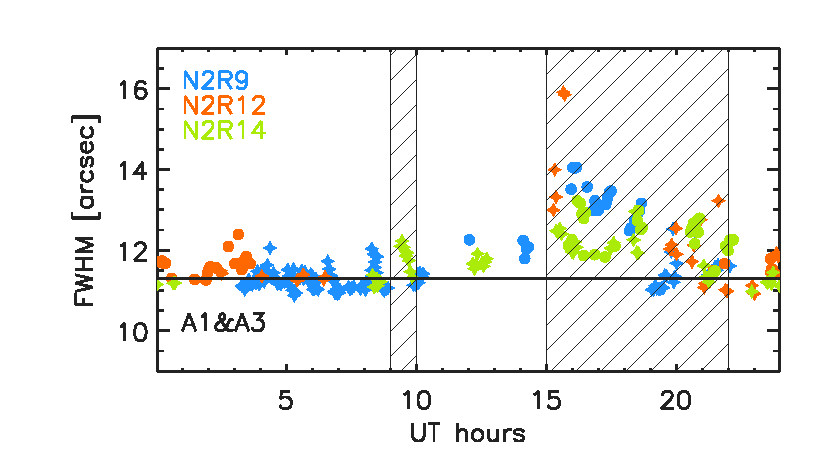
\includegraphics[clip=true, trim={0.9cm, 0.5cm, 0.5cm, 0.5cm}, width=0.4725\textwidth]{Figures/Beams/Beam_monitoring_with_otfs_vs_ut_1mm.pdf}
    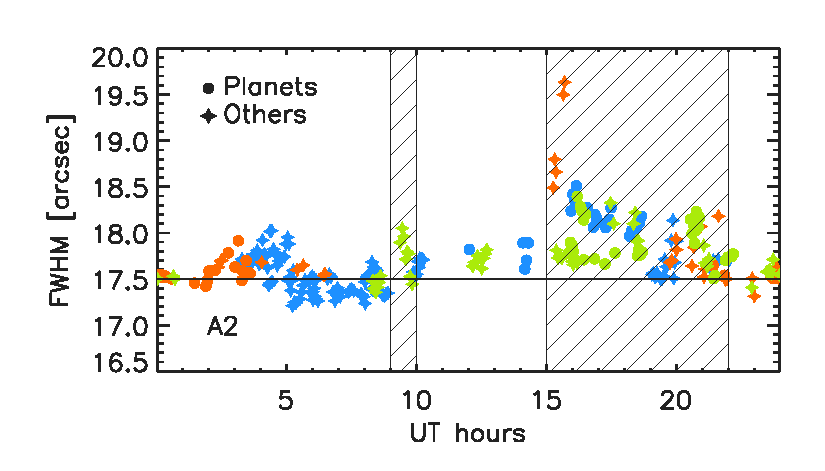
\includegraphics[clip=true, trim={0.5cm, 0.5cm, 0.5cm, 0.5cm}, width=0.4875\textwidth]{Figures/Beams/Beam_monitoring_with_otfs_vs_ut_a2.pdf}
    \caption[Beam size monitoring using OTF scans]{Beam size
      monitoring using OTF scans. FWHM at $1\,\rm{mm}$ (left panel)
      and $2\,\rm{mm}$ (right panel) as a function of the
      obsvervation time in UT hours are shown using scans of giant
      planets (filled circles) and bright point-like sources above
      $1\,\rm{Jy}$ (filled stars) for N2R9 commissioning campaign and
      N2R12 and N2R14 science pools. The cross-hatched areas
      corresponds to observing time period that are discarded using
      the baseline selection, as decribed in Sect.~\ref{se:data_selection}.} 
\label{fig:beam_monitoring_otf}
  \end{center}
\end{figure}

Figure~\ref{fig:beam_monitoring_otf} shows the geometrical FWHM as a
fonction of the observing time of the scans in UT hours for all OTF
scans of bright sources for the N2R9 commissionning campaign as well
as for the N2R12 and N2R14 science pools. For the three campaigns, we
observe the same evolution of the FWHM, which goes from a plateau at a
median value of $11.3''$ at $1\,\rm{mm}$ and $17.5''$ at $2\,\rm{mm}$
during the night, to a smooth rise that reaches a maximum of about $14''$
at $1\,\rm{mm}$ and $18.5''$ at $2\,\rm{mm}$ around 16:00 UT
hours. The beam broadening begins to become sizable around 15:00 UT
and one has to wait until around 22:00 UT for the beam sizes to lay
down on the stability plateau. The UT time ranges that are discarded
using the baseline scan selection (see
Sect.~\ref{se:data_selection}) are shown as cross-hatched areas in
Fig.~\ref{fig:beam_monitoring_otf}. They correspond to the afternoon
period between 15:00 and 22:00 UT hours, that is when the
telescope main dish is heated by daylight, as well as the
9:00-to-10:00 Sun rising period. The same beam size variations in time
using scans of giant planets (Uranus and Neptune) or other bright
sources (mainly quasars) are observed. However, FWHM from planets
observation tend to be slightly larger than FWHM from the observation
of other sources. This originates from larger 2D Gaussian fitted
values due to the error beams, which are measured with a
signal-to-noise as higher so as the source is bright. This small
effect is accounted for the beam-dependent calibration cross-check
discussed in Sect.~\ref{se:photocorr_calibration}.



\subsection{Beam monitoring using pointing}
\label{se:beam_monitoring_pointing}

As discussed in Sect.~\ref{se:pointing}, the telescope pointing is
monitored on a hour basis during observation using pointing
scans. However, as they comprize two sub-scans in azimuth and
elevation of about 10 seconds of integration time each, pointing scans
can be used to make a map of the pointing source. For each campaign,
we thus have on hand hundreds of maps of mostly point-like bright
sources. These can be also used to monitor the beam size.

%traitement pointing scans
For this purpose, pointing scans are reduced using
the data analysis pipeline described in
Sect.~\ref{se:pipeline_overview} with the same parameters as for
standard OTF scans, and projected onto maps of $2''$ resolution.
As previously, an elliptical 2D Gaussian is then fitted from the map
and a geometrical FWHM is formed from the best-fitting FWHM along the
two ellipse radii. FWHM estimates on Uranus maps are corrected for an
offset due to the finite size of the apparent disc, as discussed in
Sect.~\ref{se:beam_monitoring_otf}. Pointing scans on other extended
sources, such as NGC7027, are discarded from the analysis. 

In Fig.~\ref{fig:beam_monitoring_pointing}, we present the FWHM
estimates using pointing scans as a function of the observing time in
UT hours for three observation campaigns. We observe the same the beam
size evolution with UT hours as previously discussed in
Sect.~\ref{se:beam_monitoring_otf}, that is a plateau during night-time
and a smooth increase during day-time up to a maximum in the
afternoon, which is followed by a smooth decrease down to the plateau
a few hours after the sunset. Although the general trend is the same
as the OTF-based FWHM variations, more dispersion is seen either using
pointings toward giant planets or other bright sources.
%
\begin{figure}[ht!]
  \begin{center}
    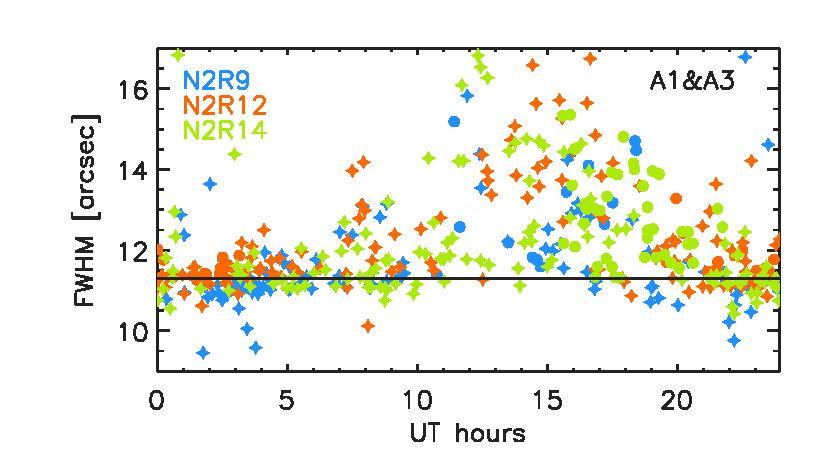
\includegraphics[clip=true, trim={0.9cm, 0.5cm, 0.5cm, 0.5cm}, width=0.4725\textwidth]{Figures/Beams/Beam_monitoring_with_pointings_vs_ut_1mm.pdf}
    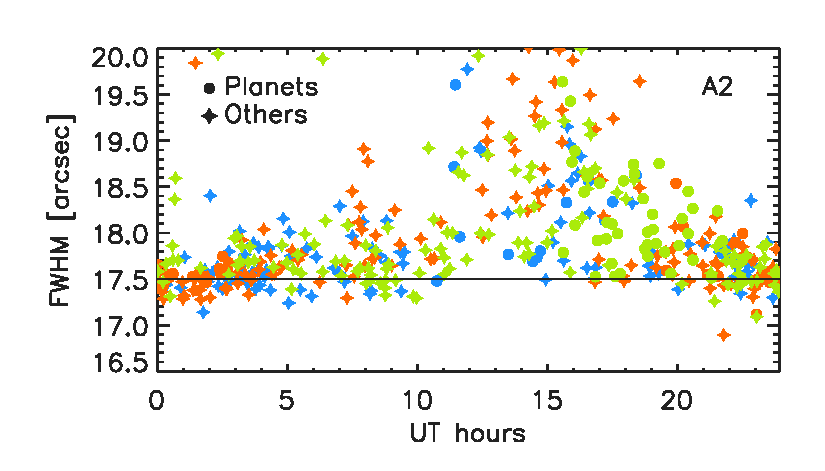
\includegraphics[clip=true, trim={0.5cm, 0.5cm, 0.5cm, 0.5cm}, width=0.4875\textwidth]{Figures/Beams/Beam_monitoring_with_pointings_vs_ut_a2.pdf}
    \caption[Beam size monitoring using pointing scans]{Beam size
      monitoring using pointing scans. Same legend as in
      Fig.~\ref{fig:beam_monitoring_otf}.} 
\label{fig:beam_monitoring_pointing}
\end{center}
\end{figure}
%
The pointing-based FWHM constitute a time-sampling of the FWHM during
the whole observation campaign. They can serve to estimate the beam
size of any observation scans, in particular
toward sources too faint for a direct FWHM fit to be made on the
projected map. To mitigate the dispersion, the time-stamped
pointing-based FWHM is filtered with a running median on a 70-minute
width time window. Then, the FWHM at the time of the considered scans is
interpolated from the smoothed pointing-based time-stamped FWHM.
%
\begin{figure}[ht!]
  \begin{center}
    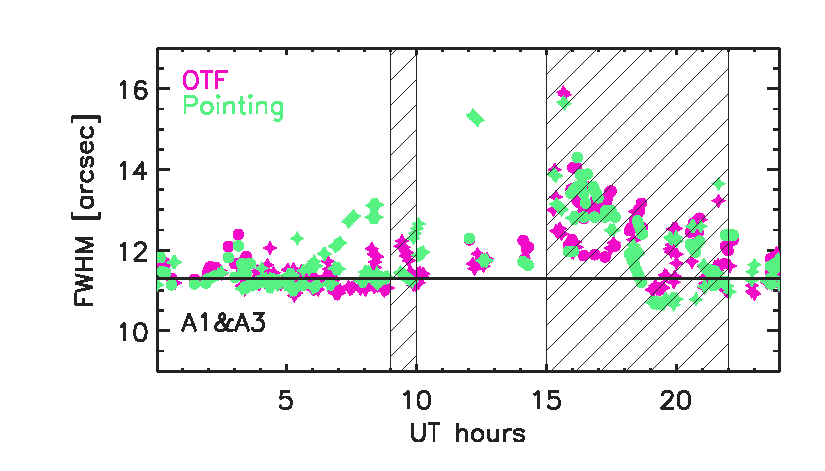
\includegraphics[clip=true, trim={0.9cm, 0.5cm, 0.5cm, 0.5cm}, width=0.4725\textwidth]{Figures/Beams/Beam_monitoring_with_otfs_vs_ut_compare_pointings_1mm.pdf}
    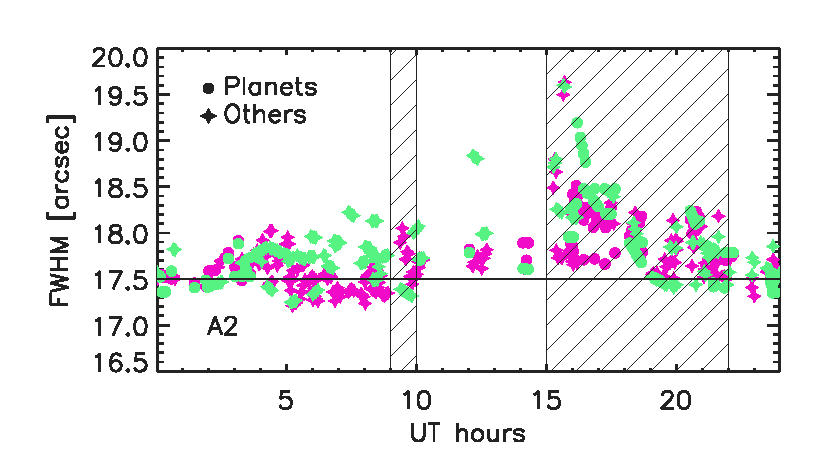
\includegraphics[clip=true, trim={0.5cm, 0.5cm, 0.5cm, 0.5cm}, width=0.4875\textwidth]{Figures/Beams/Beam_monitoring_with_otfs_vs_ut_compare_pointings_a2.pdf}
    \caption[Beam size monitoring comparison]{Beam size monitoring
      comparison. The FWHM estimates from a 2D Gaussian fit on the map
      of OTF scans toward bright sources ('OTF'-labeled pink data
      points) are compared to FWHM estimates that are obtained by
      interpolating the smoothed pointing-based FWHM at the time of
      the scans ('Pointing'-labeled light green data points).}
\label{fig:beam_monitoring_compare}
\end{center}
\end{figure}
%
Figure~\ref{fig:beam_monitoring_pointing} shows two different FWHM
estimates for the same data set: the best-fitting FWHM estimates on
the map are compared with the interpolation from the pointing-based
FWHM monitoring. The two estimates are well in agreement with each
other, although the pointing-based estimates have more dispersion and
a few outliers.\\

As a summary, we have evidenced a systematic beam size variation with
the observation time using two different data sets: a series of OTF
scans of bright sources and pointing scans. The beam size
variation is i) reproducible from a campaign to another, stable
with ii) the data set and iii) the sources. It consists of a beam
broadening during afternoons, as the $30\,\rm{m}$ dish is heated by
the daylight, and
an increase of the dispersion during sunrises. The most impacted
observing periods are well discarded using the baseline selection
criteria discussed in Sect.~\ref{se:data_selection}.





%% [Full beam pattern]
%%________________________________________________________
\section{Full beam pattern {\color{blue} Laurence}}
\label{se:fullbeam}

\subsection{Data sets}
\label{se:beammap_set}

The characterization of the IRAM $30\,\rm{m}$ beam pattern observed
through NIKA2 detectors is mainly based on observations of strong
compact sources, such as planets including Uranus, Neptune and Mars,
and bright quasars. We generally use \bm\ scans, which we recall,
are deep-integration raster-scan observations that consist of 99
sub-scans placed at intervals of $4.8''$ to cover a total of $13.5'
\times 7.8'$ (see also Sect.~\ref{se:beammaps}). Most of our
beam-related analysis are beased on the same
set of \bm\ scans as previously selected to perform the average
FOV reconstruction, as presented in Sect.~\ref{se:fp_reconstruction}.
The set comprises nine \bm\ scans that distribute as one from N2R8,
'20170125s243',
two from N2R9,
'20170224s177' and '20170226s415' and six from N2R10, which are
'20170226s425', '20170227s84', '20170419s133', '20170420s113',
'20170424s116', '20170424s123'.



\subsection{Deep beam maps}
\label{se:beammaps}
We present the two-dimensional distribution of the beam in
Fig.~\ref{fig:beam}. We primary use a map obtained from a combination
of deep observations of strong point sources collected during
\emph{NIKA2-run8} and \emph{run9}. Namely, we use 'beammap' OTF scans
of Uranus (scan id '20170125s223' and '20170125s243'),  Neptune
('20170224s177') and the bright quasar 3C84 ('20170226s415'). However,
we checked the stability of our results on single scan maps,
combinations of scans for a single source, and combinations of
shallower scans but spanning a large range of scanning direction. The
data processing includes a mitigation of the correlated noise, which
mainly originates from the atmosphere.  We primarly use a subtraction
of a common mode estimated from the most correlated detectors (the
so-called 'cm one block' method). However, other methods are tested
for assessing the immunity of our results to noise residuals.

\begin{figure}[ht!]
\begin{center}
  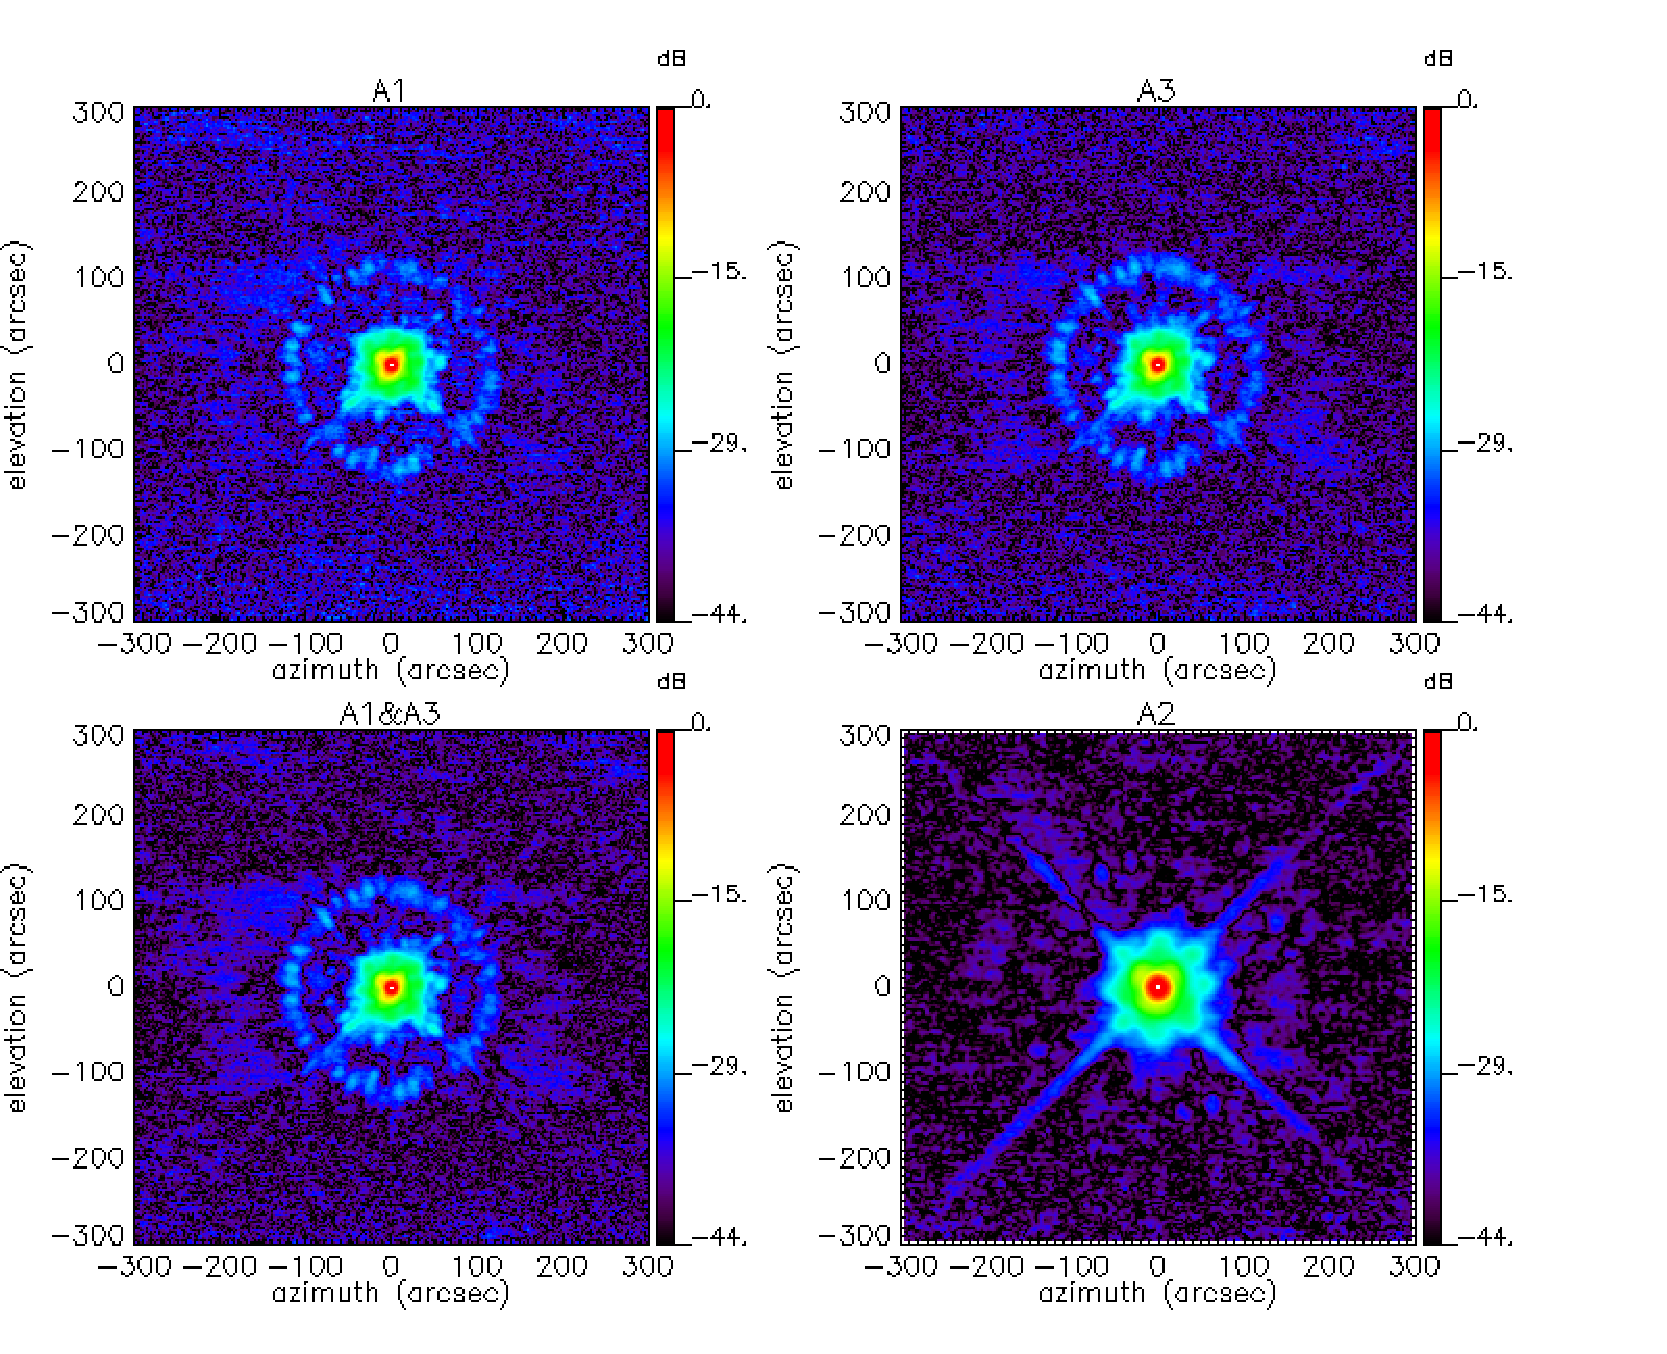
\includegraphics[clip, angle=0, scale=0.4]{Figures/Lobe_map_Combo_v2_dB.pdf}
 \caption[Beam pattern.]{From upper left to lower right, beam maps of array 1 (labeled 'A1'), array 3 ('A3'), the combination of the 1.15mm arrays ('A1$\&$3') and the 2mm array ('A2') are shown in decibel. These maps, which consist of normalized combination of four long OTF scans of bright point sources, are in celestial coordinates and cover a sky area which extend over 10 arcmin.}
\label{fig:beam}
\end{center}
\end{figure}

The deep NIKA2 beam maps reveal some noticeable features, which are
shown in Fig.~\ref{fig:features} and which comprize:
\begin{itemize}
\item[(1)] four symmetrical spokes of the error beam as shown by
  yellow arrows in the A2 panel, which are expected from \emph{Zemax}
  simulations;
\item[(2)] shallow spikes of unknown origin, which are circled by pink
  ellipses. The multiple images on the combined deep beam map indicate
  a rotation of these spikes with the observing elevation, which in
  turn point to diffraction related issue or a ghost image that are
  formed inside the cryostat;
\item[(3)] other spikes of unknown origin, as pointed with the yellow
  arrows in the A3 panel. The ones that are close to the vertical and
  horizontal radii are reproduced by 'Zemax' simulation but with a  
  shallower, whereas the ones in the diagonal directions may be due to
  external calibrator installed close to the secondary mirror.  
\end{itemize}

\begin{figure}[ht!]
\begin{center}
  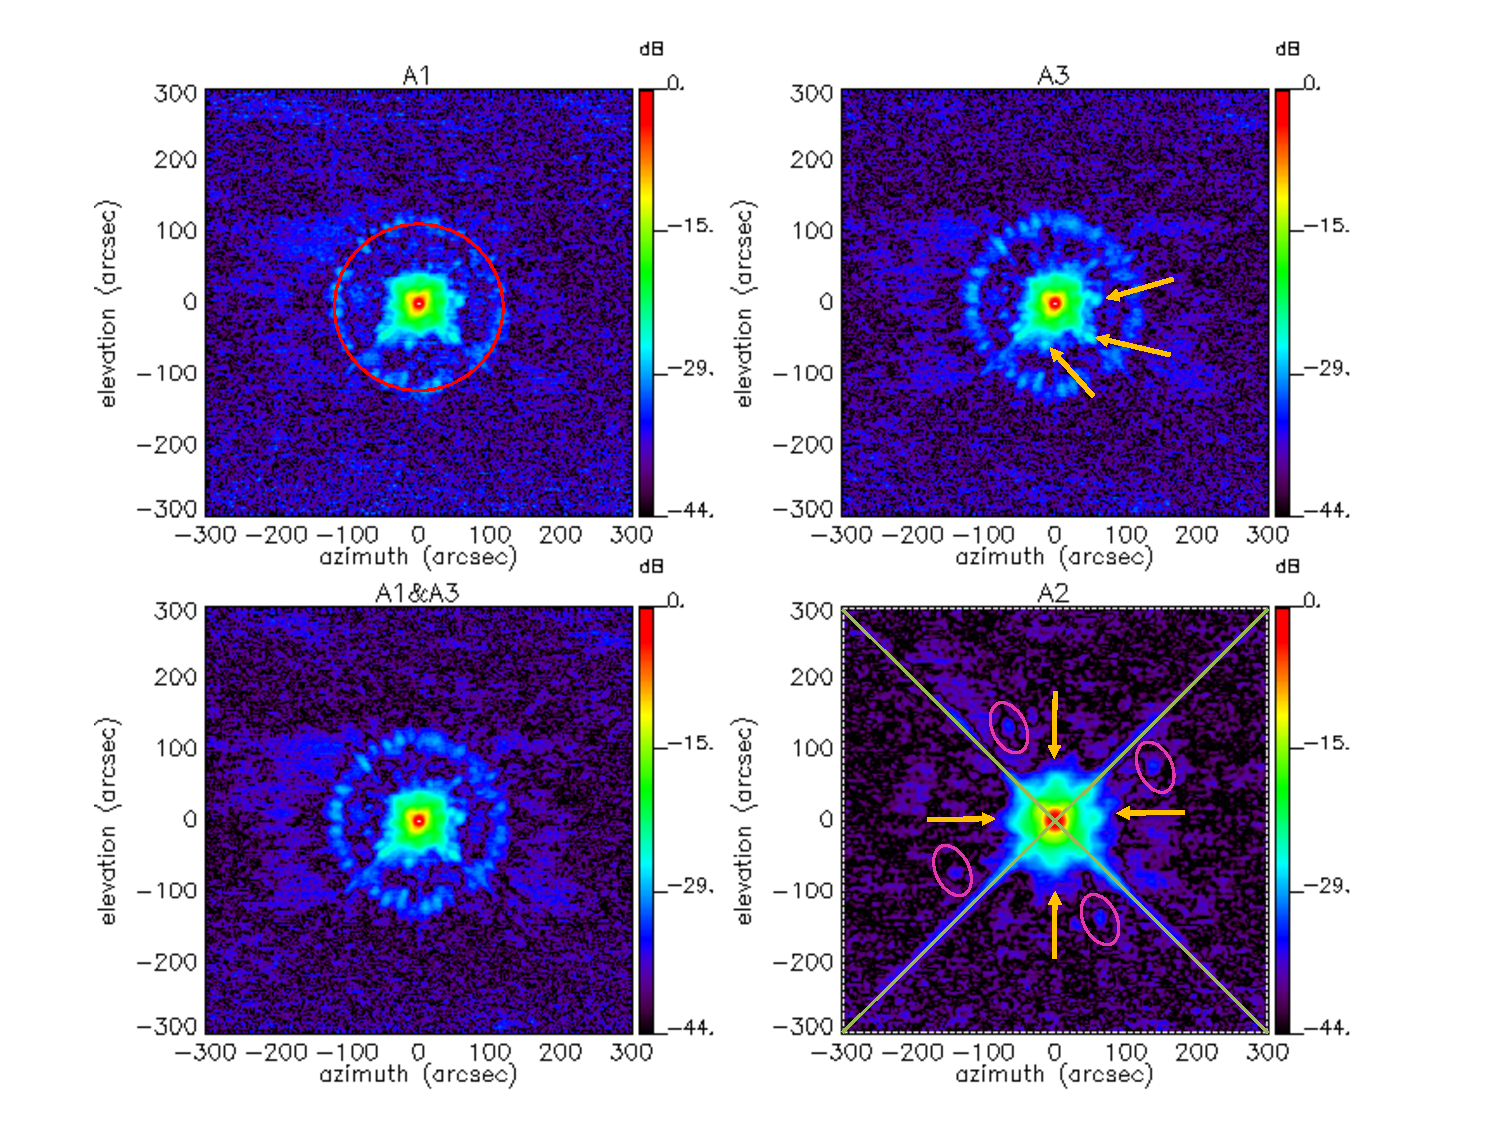
\includegraphics[clip, angle=0, scale=0.4]{Figures/Beams_features.pdf}
\caption[Noticeable features of NIKA2 beam pattern.]{ Red circle: diffraction ring seen in 1-mm maps (the spokes are presumably caused by radial and azimuthal panel buckling (cf. Fig.4 in Greve et al. 2010)); Perpendicular green lines: diffraction pattern caused by quadrupod secondary support structure (prominently seen in 2mm maps); Yellow arrows in the upper right pannel: pattern of 3 spikes seen in 1mm maps of unknown origin; Yellow arrows in the lower right pannel: four symmetrical spokes of the first errorbeam; Pink ellipses: 4 spikes seen in 2mm maps.}
\label{fig:features}
\end{center}
\end{figure}


To gain a first impression of the structure of the Iram 30-m beam as
seen with NIKA2, we use radial cuts to evidence the relative level of
the main beam, the first error beam and other features seen in the 2D
beam pattern using radial cuts. NIKA2 full beam is shown in the left
panels of Fig.~\ref{fig:beam_structure_example} by means of two
orthogonal cuts through Uranus from a high quality map obtained on
2017 January 25th in excellent conditions
(low opacity $\tau_{225}=0.08$ and elevation $46^{\circ}$).


\begin{figure}[ht!]
  \begin{center}
    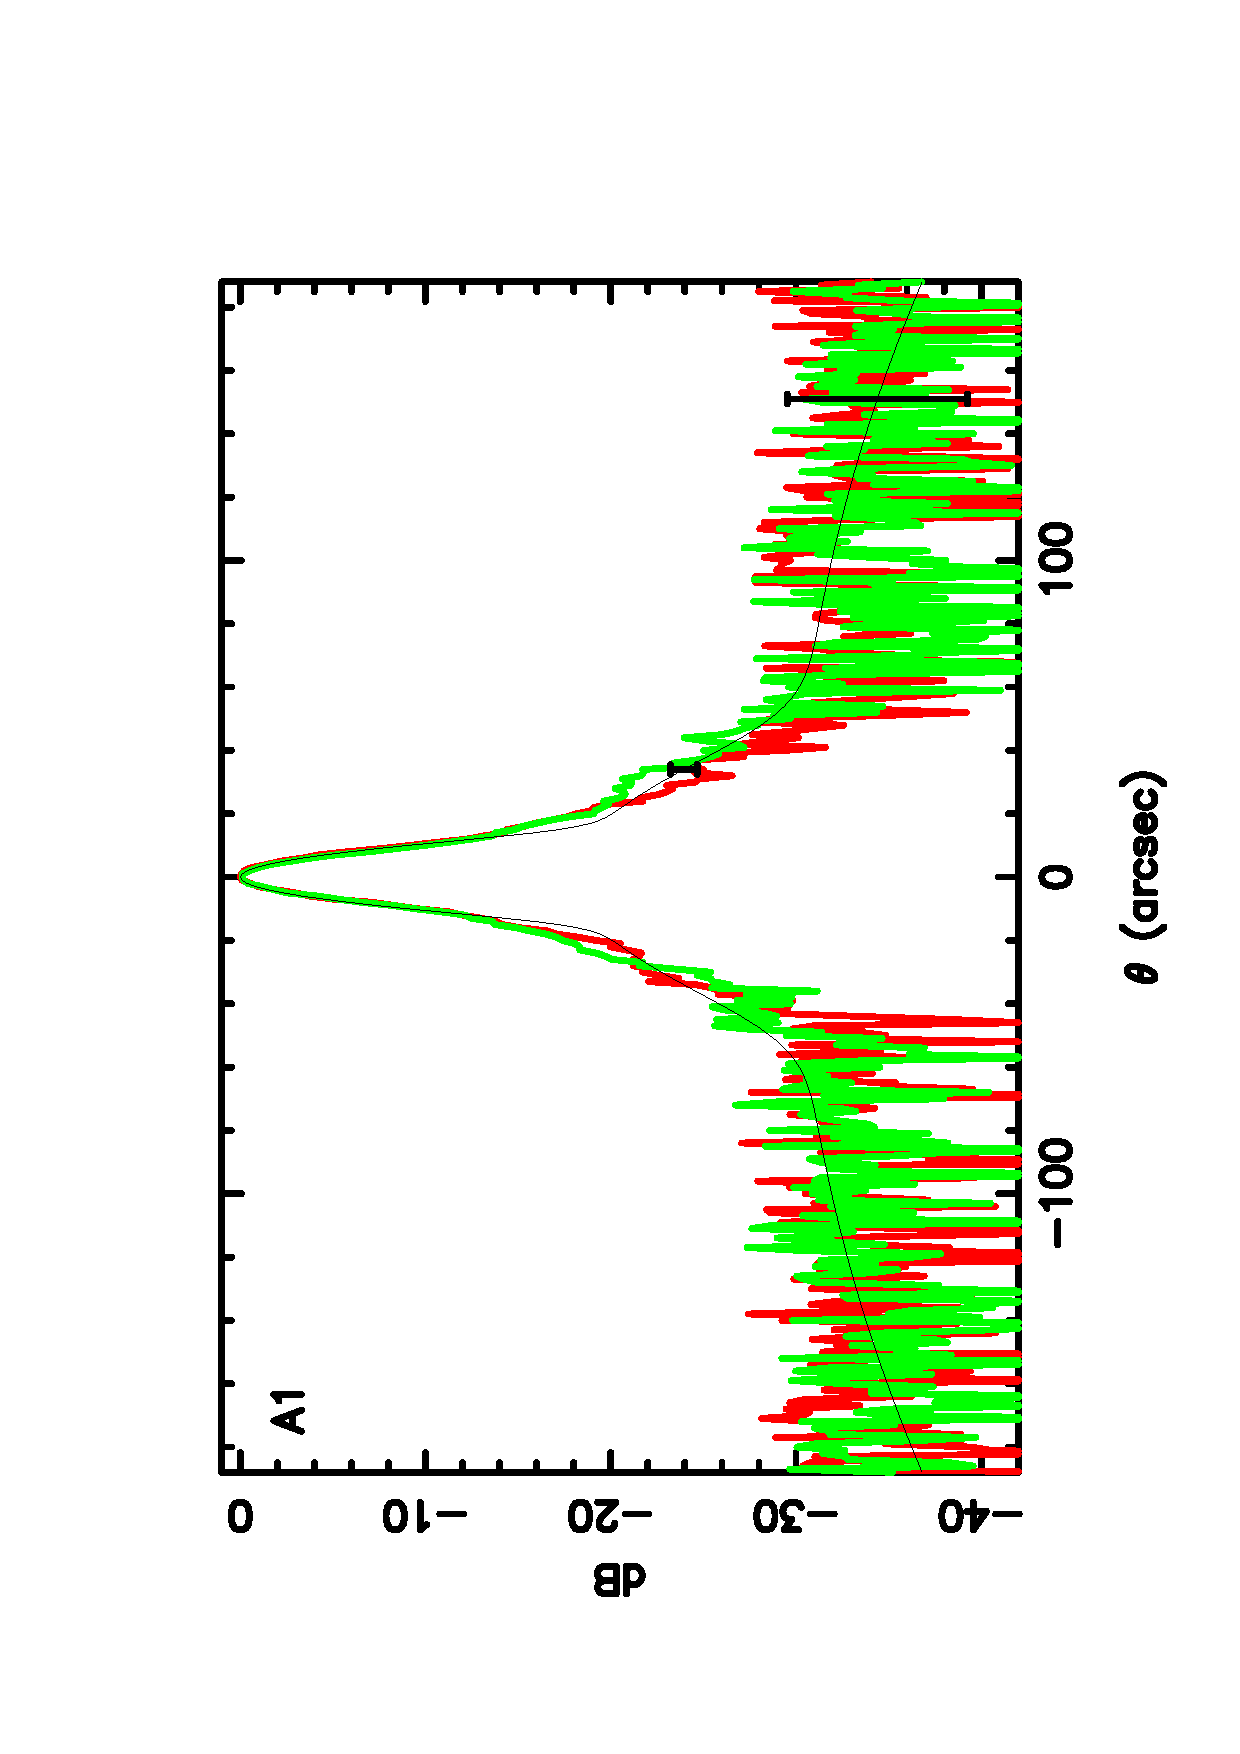
\includegraphics[clip=true, width=0.39\textwidth]{Figures/Array_A1_dB.pdf}
    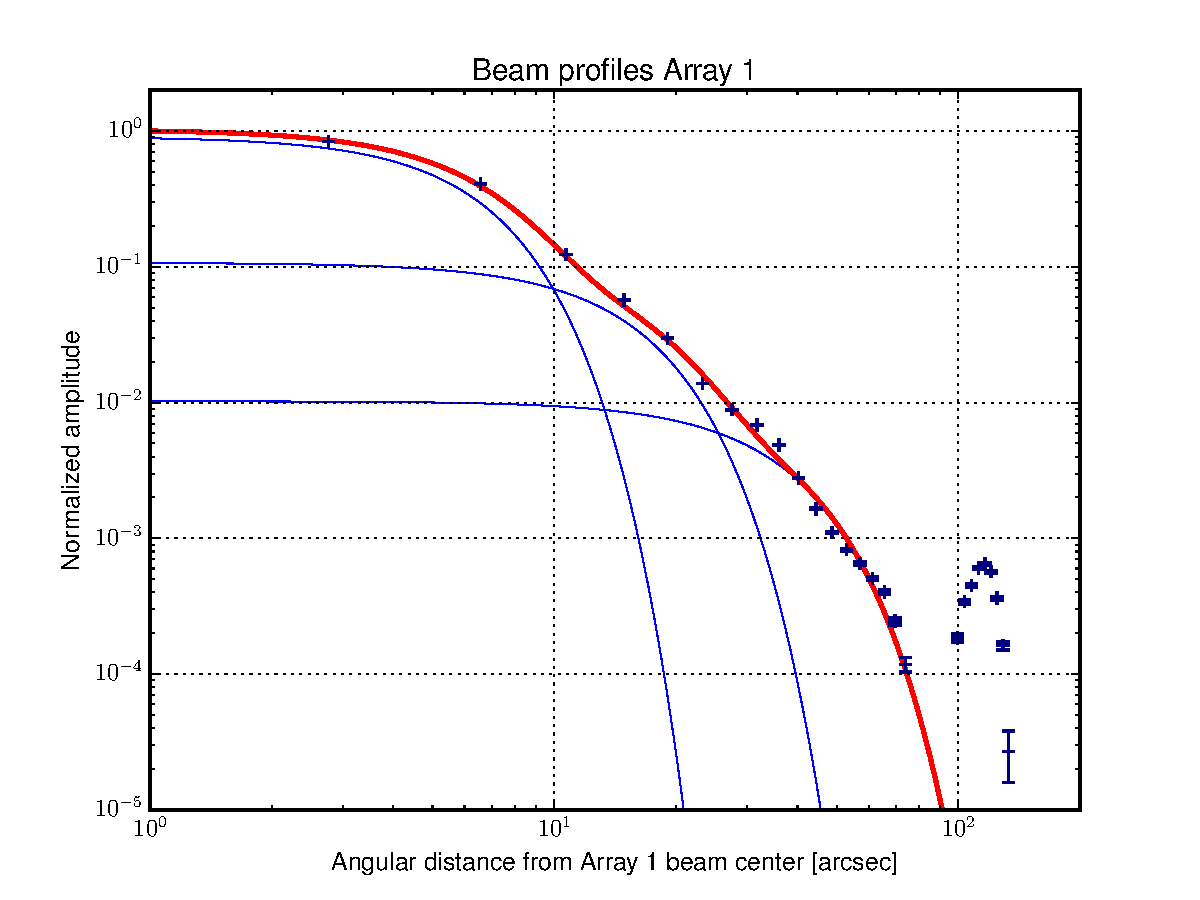
\includegraphics[clip=true, trim={-0.5cm, -0.65cm, 0, 0}, width=0.44\textwidth]{Figures/Beam_profiles_A1_FR.pdf}
    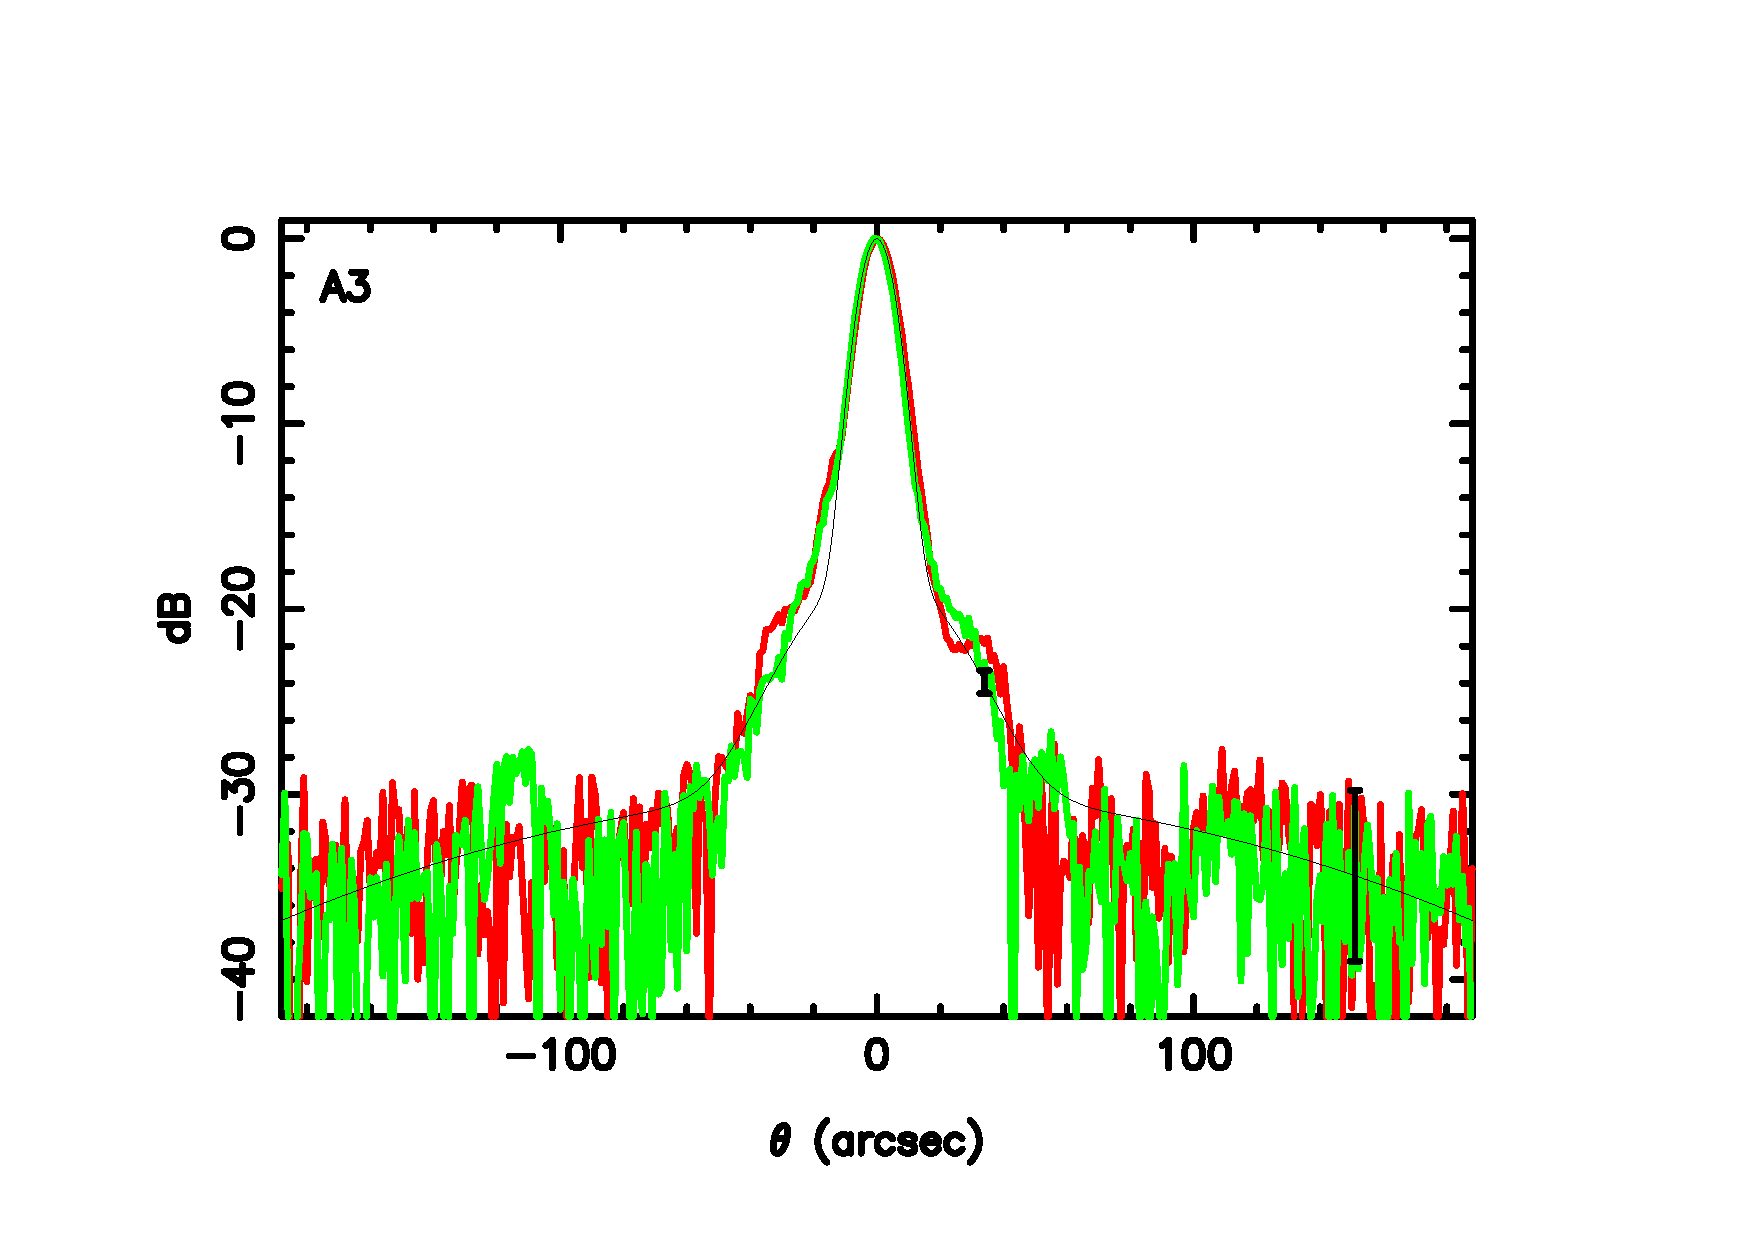
\includegraphics[clip=true, width=0.39\textwidth]{Figures/Array_A3_dB.pdf}
    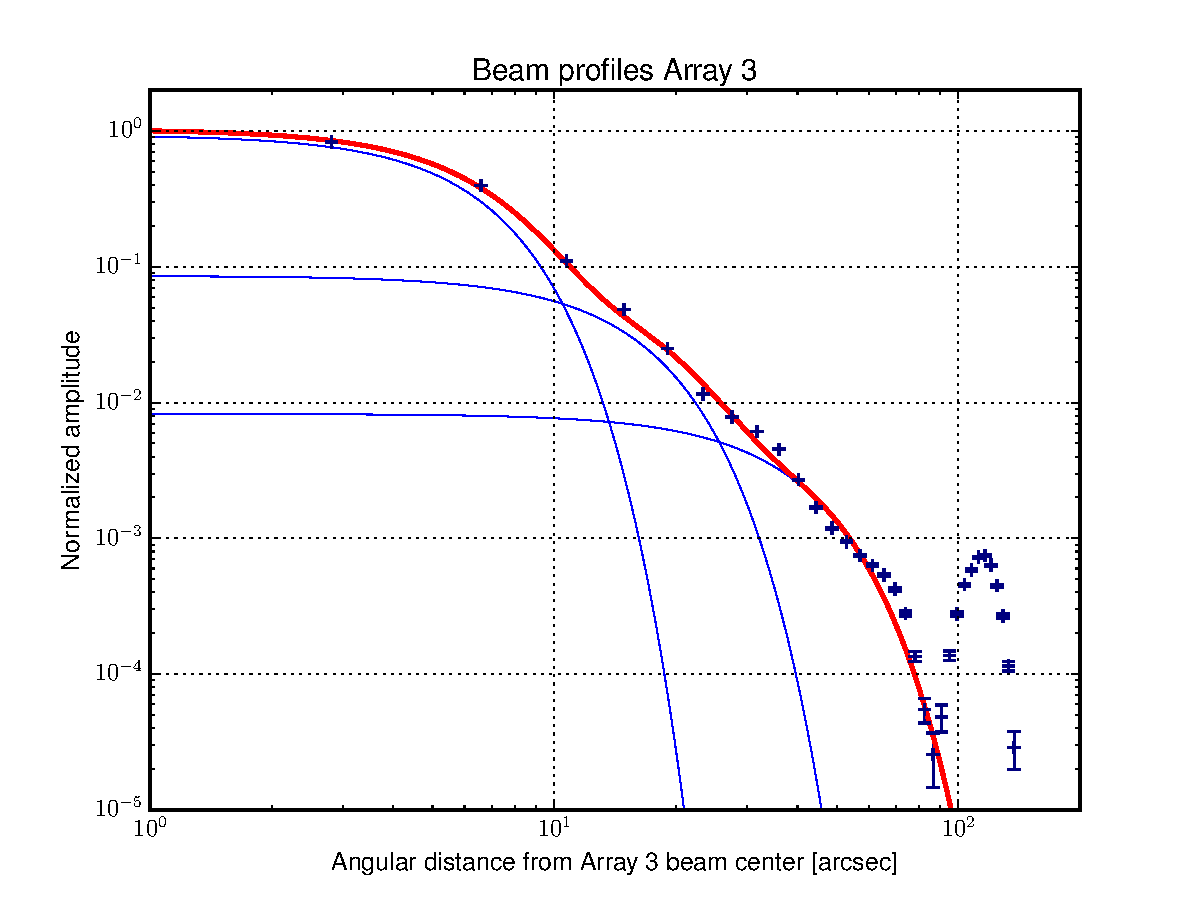
\includegraphics[clip=true, trim={-0.5cm, -0.65cm, 0, 0}, width=0.44\textwidth]{Figures/Beam_profiles_A3_FR.pdf}
    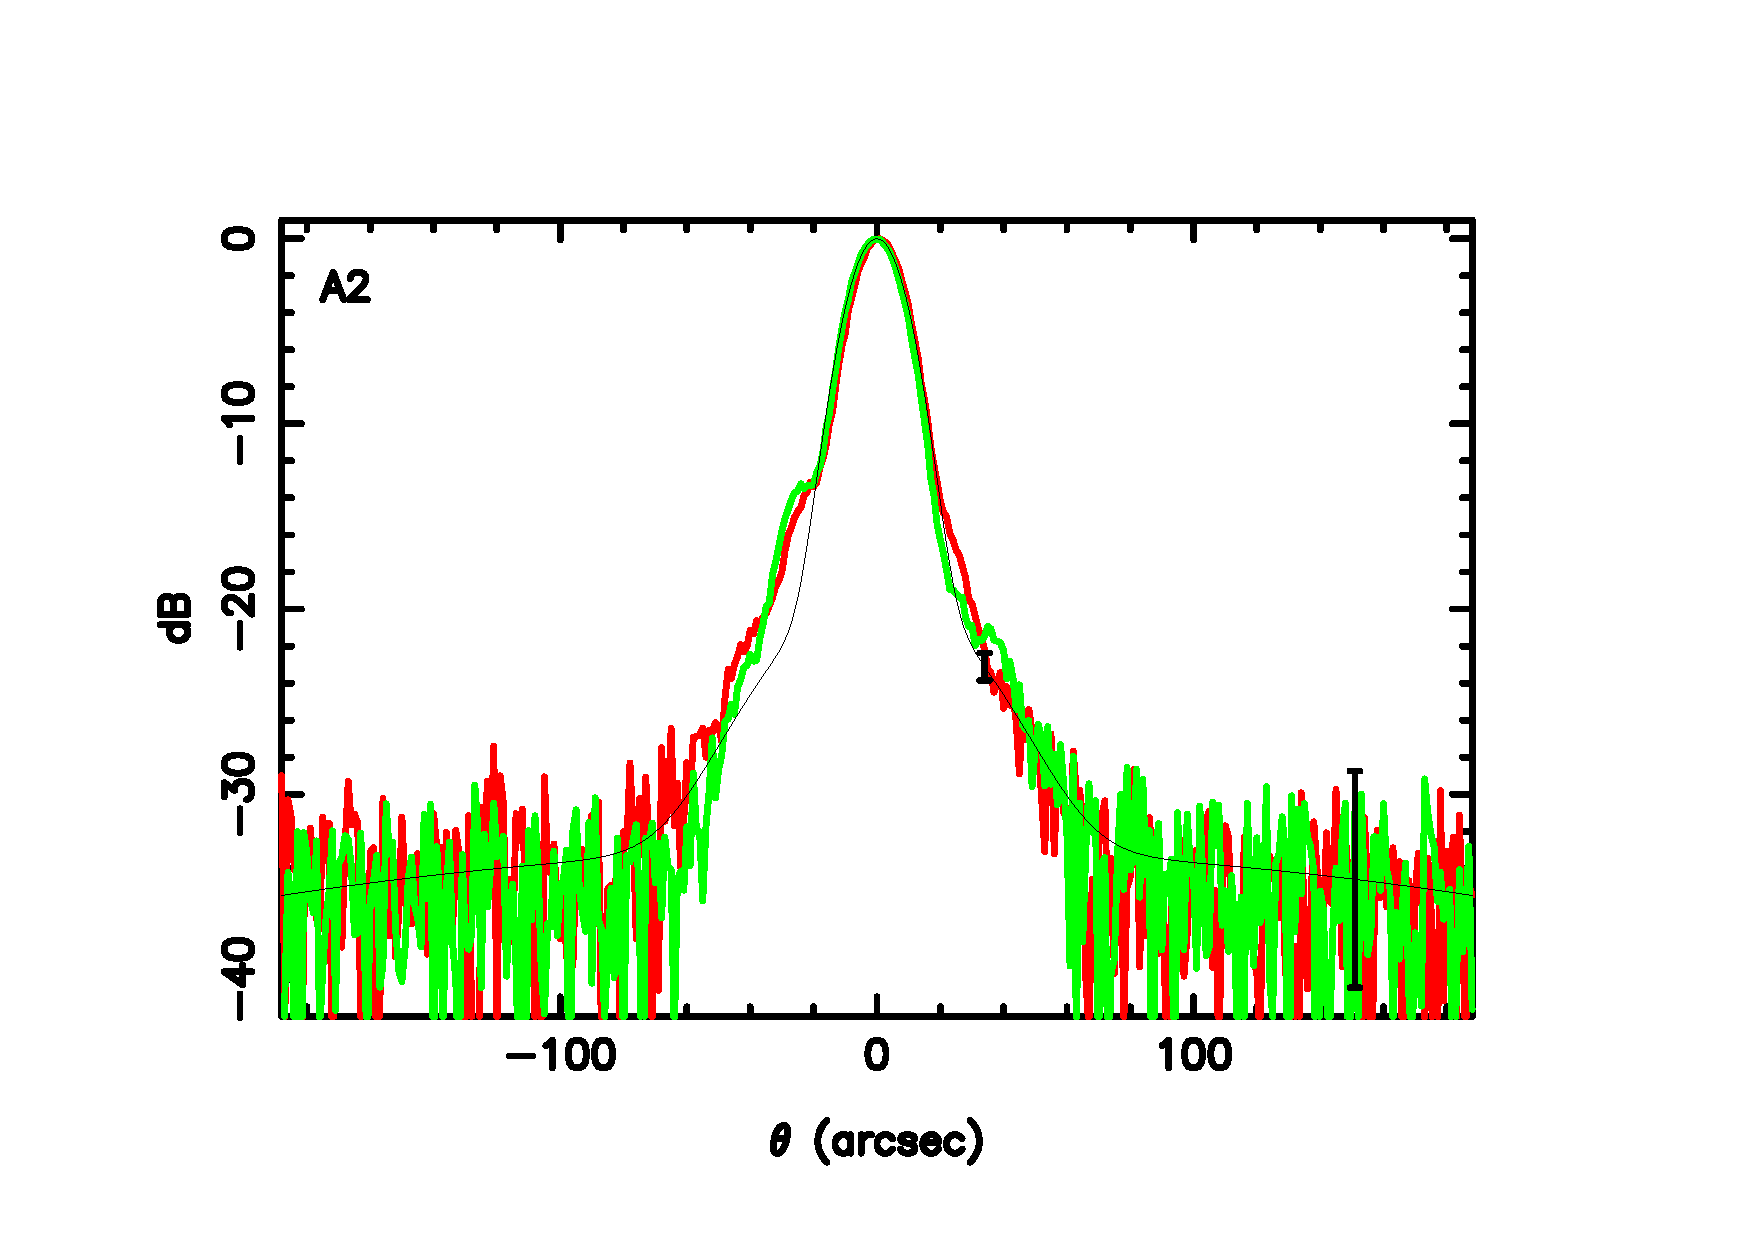
\includegraphics[clip=true, width=0.39\textwidth]{Figures/Array_A2_dB.pdf}
    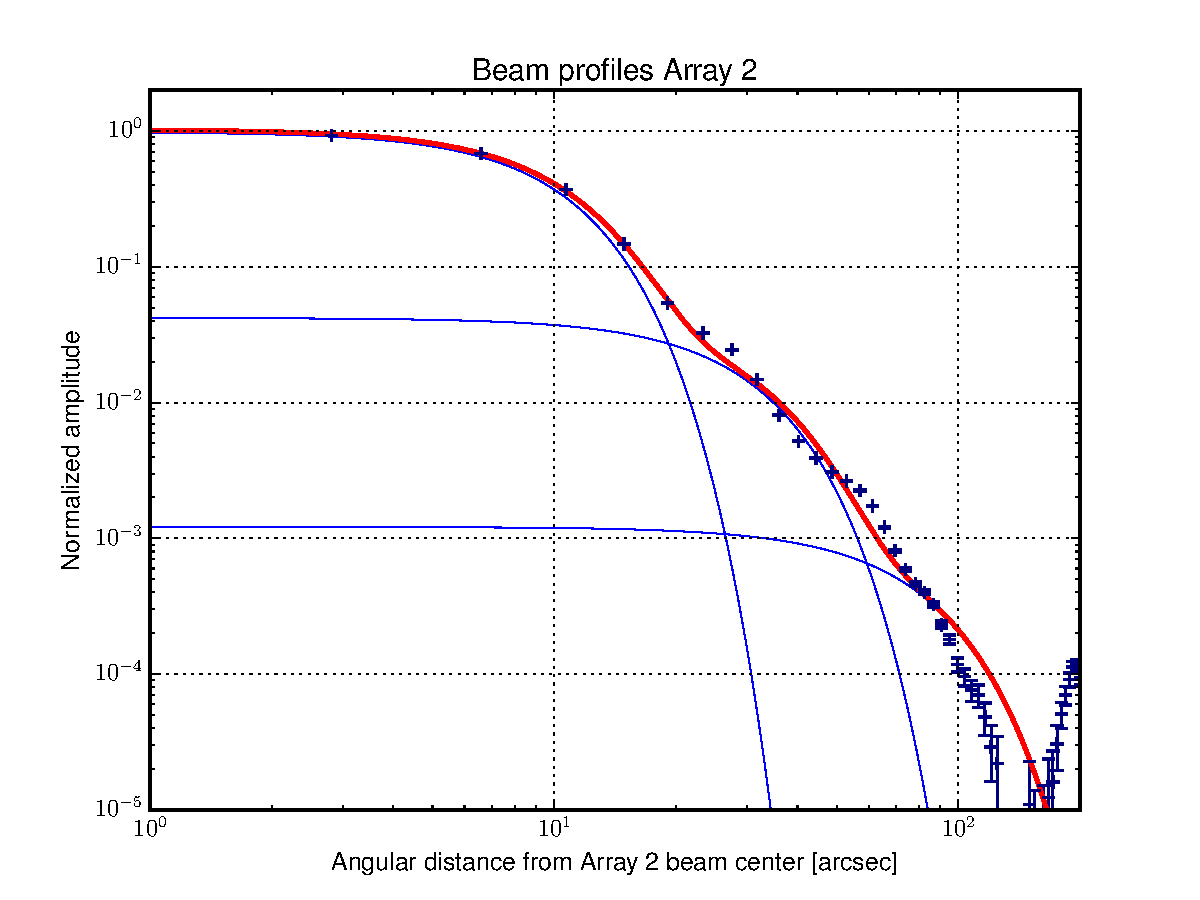
\includegraphics[clip=true, trim={-0.5cm, -0.65cm, 0, 0}, width=0.44\textwidth]{Figures/Beam_profiles_A2_FR.pdf}
    \caption[Beam structure]{\emph{Left column:} Two orthogonal cuts through the
      beam are shown in red and green and a best fit model made of three
      Gaussians is superimposed in black.
      These cuts were obtained from the high quality map of Uranus on 2017
      January 25th. The main beam starts to depart from the first Gaussian
      at -12dB. \emph{Right column:} Example of beam radial profile
      estimated on the same map of Uranus. The Best-fitting curve is show
      in red using a three Gaussian model.   
    }
    \label{fig:beam_structure_example}
    %\label{fig:beam_profiles_3G}
  \end{center}
\end{figure}

A model made of three Gaussians centered on the source peak was best
fit {\it by hand} to these cuts.
%the parameters are reported in Table \ref{tab:3gauss} [PEUT-ETRE
%AVANTAGEUSEMENT REPLACED PAR VALEURS DE FLORIAN].
We observe that the main beam starts to depart from the first
Gaussian at the level of about -12dB for the three arrays.
We note that for the instrument EMIR on the radiotelescope,
this departure is about -20dB (Kramer, Penalver and Greve
2013). However, this
discrepancy between a feedhorn-based experiment and a bare pixels one
is expected since the main effect of the feedhorns is to lower the
side lobes of the Airy diffraction pattern.
The precise characterization of the full beam structure is discussed
in Sect.~\ref{se:fullbeam_prof}.  

%From parameters in Table \ref{tab:3gauss}, one can estimate that
%the source incident power is split about equally between the main beam
%and the error beam at 1mm, and these fractions are 70\% and 30\% at 2mm, respectively.
%This modelling uses the central
%region   $180'' \times 180''$ in size with a uniform noise rms from
%a larger area of 8' x 5' on the sky scanned with the arrays. It is expected
%that the error beam extend beyond these limits.


%\begin{table}
%\centering 
%\caption[]{Model parameters of the three Gaussian beam.}
%\begin{tabular}{|l|l|l|l|l|l|l|}
%\hline
%               & \multicolumn{3}{c|}{A1 and A3} & \multicolumn{3}{c|}{A2}  \\
%\hline
%fwhm      & $11.25''$ & $45''$  & $250''$ & $17.75''$ & $56''$  & $420''$ \\
%amplitude & 0.984     & 0.015   & 0.0005   &  0.9875   & 0.011   &  0.0005\\
%\hline
%\end{tabular}
%\label{tab:3gauss}
%\end{table}


\subsection{Beam profile}
\label{se:fullbeam_prof}

{\bf complete this sub-section}

The beam profile is the azimuthal average of the beam map around the
main beam center. Although the profile cannot represent the sub-dominant non-axisymetrical
extended features, which are seen in the beam pattern and discussed in
Sect.~\ref{se:beammaps} (telescope arms, spikes), it provides us with a useful
representation of the internal and central parts of the beam (about up to
$100''$). We determine a beam profile from a beam map in centering to
the fitted value of the main beam center and forming the
weighted average of the pixels equidistant to the center.

We model the beam profile as a three-Gaussian function defined as:
\begin{equation}
  B(\theta) = \sum_i A_i G_i(\theta) + B_0
\end{equation}

Right panels of Fig.~\ref{fig:beam_structure_example} shows the beam
profile from a beam map acquired during {\emph N2R8} (scan ID:
20170125s223), as well as the best-fit 3-Gaussian model. 




%%%%%%%%%%%%%%%%%%%%%%%%%%%%%%%%%%%%%%%%%%%%%%%%%%%%%%%%%%%%%%%%%
% Stability of the beam pattern
We checked the stability of the beam against various observing
condition (source intensity, weather condition, focus optimisation) by
comparing the beam profile of the beam-map set, which comprizes nine
beam-maps acquired from N2R8 to N2R10, as defined in
Sect.~\ref{se:beammap_set}.
The nine beam profiles and their ratio
w.r.t. the median beam profile are shown in Fig.~\ref{fig:beam_prof}.


\begin{figure}[ht!]
  \centering
  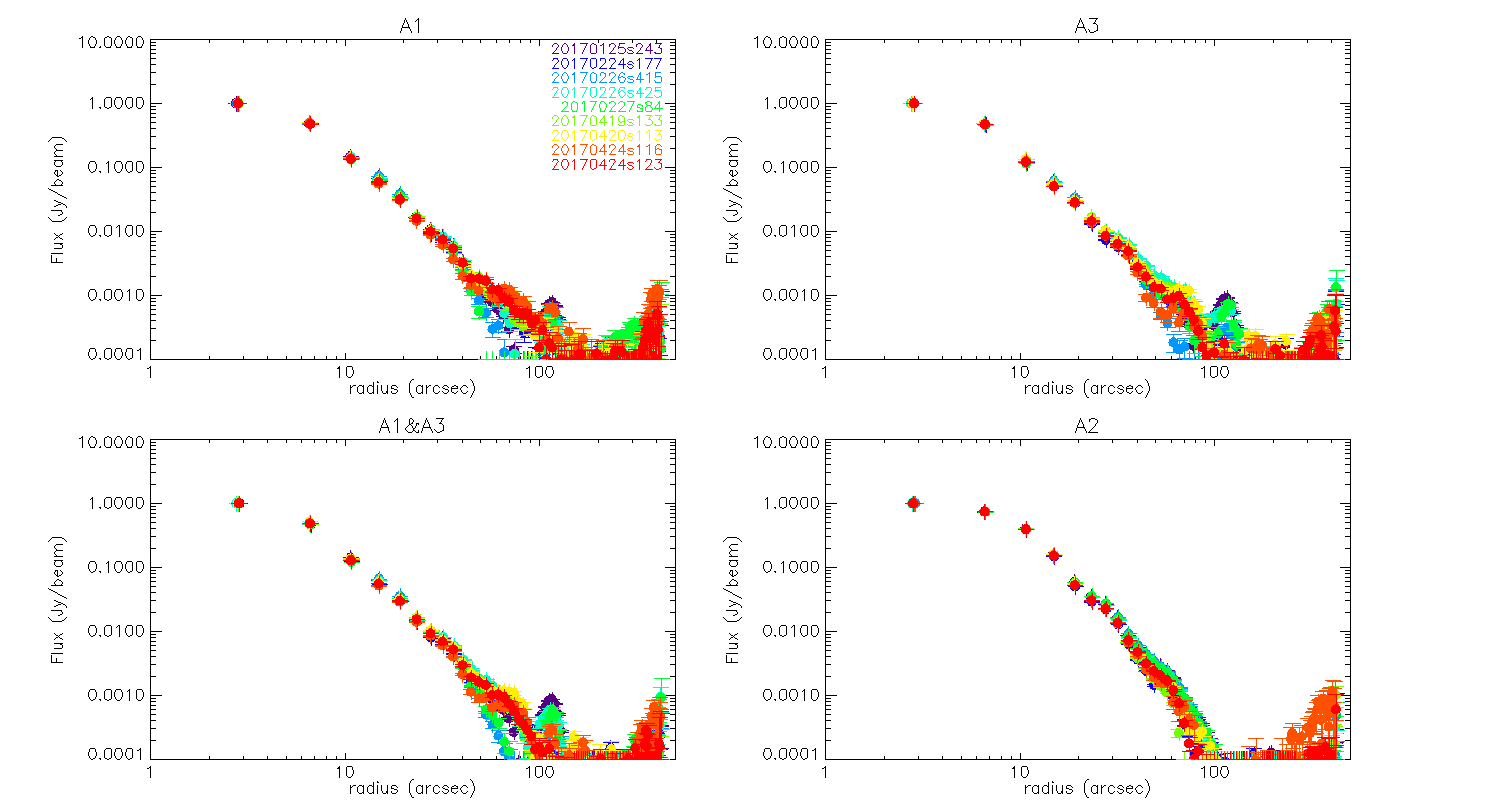
\includegraphics[clip=true,width=\textwidth]{Figures/Profile_allscans_mixed}
  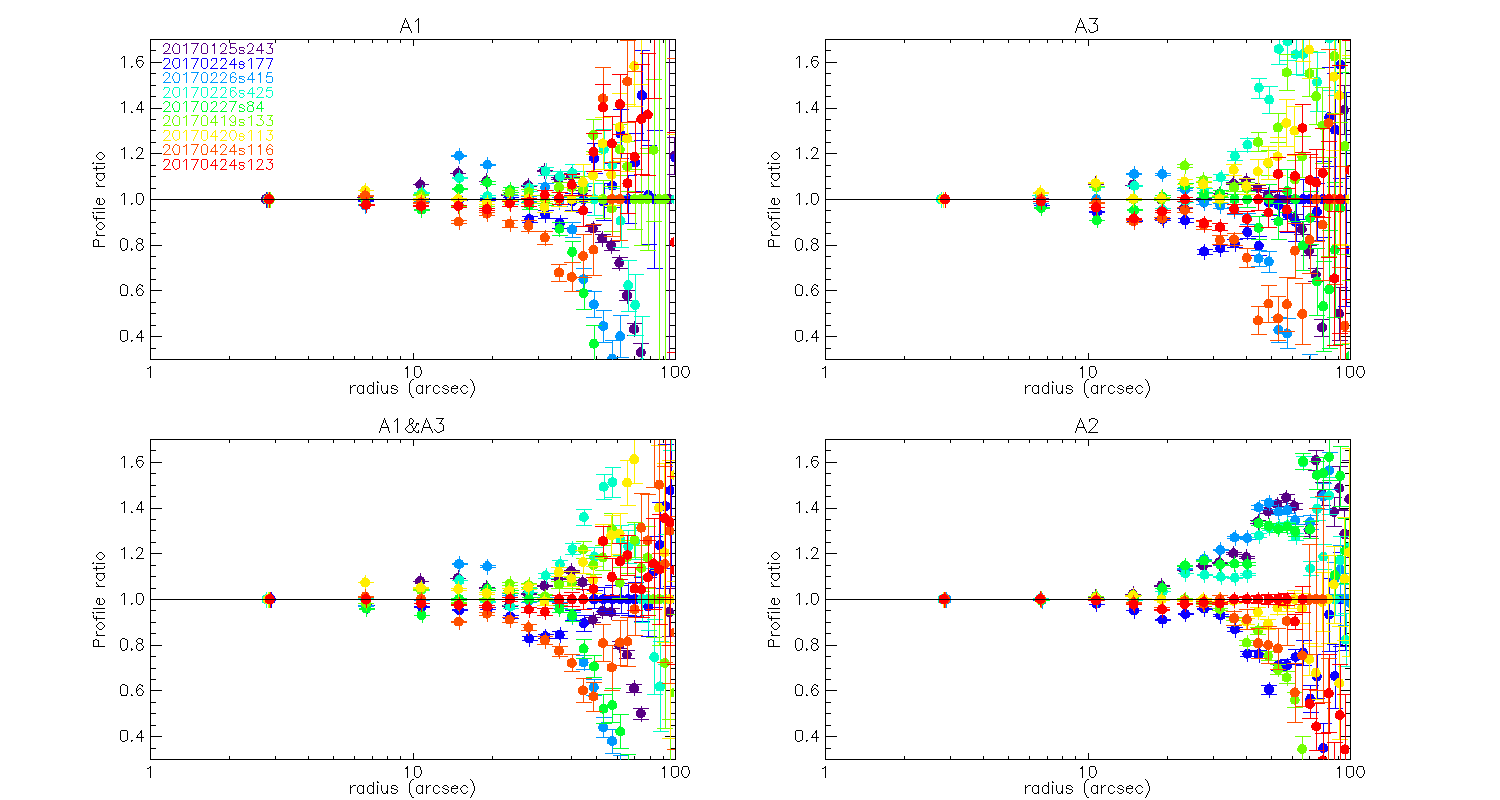
\includegraphics[clip=true,width=\textwidth]{Figures/Profile_allscans_over_median_mixed}
\caption[Stability of the beam profile]{Beam profiles from various N2R8 to N2R10
  beam-map scans. The upper panel shows the beam profiles normalised
  to the maximum value, and the lower panel the ratios w.r.t. the median profile.}
  \label{fig:beam_prof}
\end{figure}

